\section{Heaps}

\begin{description}
	\item [Heap] Nearly complete binary tree.  All levels, except perhaps the lowest, are complete, and the bottom row is filled from the left.  
	\item [Max-heap property] $A[Parent(i)] \ge A[i]$ The children are no larger than their parent.  
	\item [Min-heap property] $A[Parent(i)] \le A[i]$ The children are no less than their parent.  
\end{description}

\

Max-heap $\{16,14,10,8,7,9,3,2,4,1\}$ as a binary tree.  

\

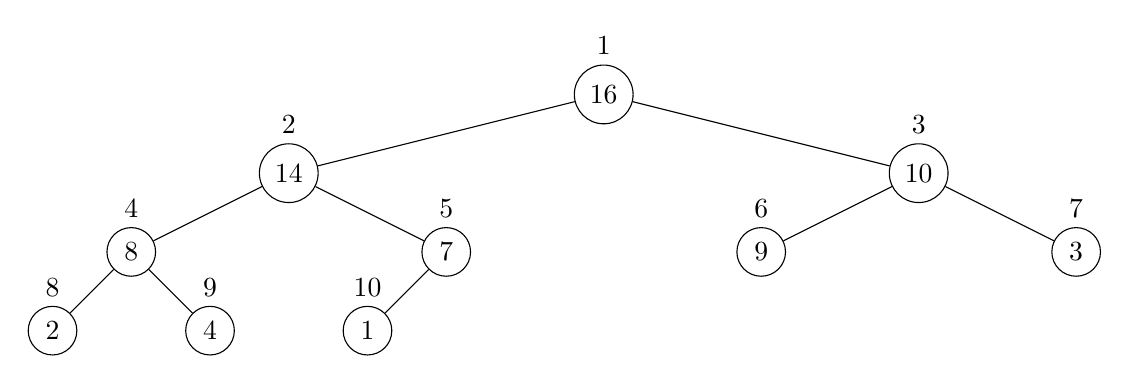
\begin{tikzpicture}[x=10mm, y=10mm]
	\node [circle, draw, label=above:1] (1) at (0,0) {16};
	\node [circle, draw, label=above:2] (2) at (-4,-1) {14};
	\node [circle, draw, label=above:3] (3) at (4,-1) {10};
	\node [circle, draw, label=above:4] (4) at (-6, -2) {8};
	\node [circle, draw, label=above:5] (5) at (-2,-2) {7};
	\node [circle, draw, label=above:6] (6) at (2,-2) {9};
	\node [circle, draw, label=above:7] (7) at (6,-2) {3};
	\node [circle, draw, label=above:8] (8) at (-7,-3) {2};
	\node [circle, draw, label=above:9] (9) at (-5,-3) {4};
	\node [circle, draw, label=above:10] (10) at (-3,-3) {1};
	\foreach \from/\to in {1/2,1/3,2/4,2/5,3/6,3/7,4/8,4/9,5/10}
		\draw (\from) -- (\to);
\end{tikzpicture}

\

Building a max heap takes $O(n)$ time.  

If you have built a max heap and swap out the root node, then it takes $O(\lg n)$ steps to restore the heap.  

Since the head node of a max heap is always the largest node, a method that works to sort the heap is to take out the head node, replace it with the last node, restore the heap, and repeat until the heap is empty.  Since this sort takes $n-1$ steps, and each step takes $O(\lg n)$ time, the sort takes $O(n \lg n)$ time.  

%%%%%%%%%%
\subsection{Old Exam Questions}

%%%%%
\subsubsection{Spring 2019 \#L4}
	% S19 #L4
	The Dijkstra's algorithm (DIJ) solves the single-source shortest-path problem in a weighted directed graph $G=(V,E)$.  Given the graph $G$ below, follow DIJ to find shortest paths from vertex $s$ to all other vertices, with all predecessor edges shaded and estimated distance values from $s$ to all vertices provided at the end of each iteration.  
	
	What is the time complexity of DIJ for a general graph $G=(V,E)$, if the candidate vertices are kept in a binary min-heap?
		
	
\

\hfil \begin{tikzpicture}[x=20mm, y=15mm]
	\node [circle, draw] (s) [label=left:{s}] at (0,0) {$0$};
	\node [circle, draw] (t) [label=above:{t}] at (1,1) {$\infty$};
	\node [circle, draw] (x) [label=above:{x}] at (3,1) {$\infty$};
	\node [circle, draw] (y) [label=below:{y}] at (1,-1) {$\infty$};
	\node [circle, draw] (z) [label=below:{z}] at (3,-1) {$\infty$};
	\draw[-triangle 60] (s) to node[circle, fill=white, midway]{10} (t);
	\draw[-triangle 60] (s) to node[circle, fill=white, midway]{5} (y);
	\draw[-triangle 60] (t) to node[circle, fill=white, midway]{1} (x);
	\draw[bend right=20, -triangle 60] (t) to node[circle, fill=white, midway]{2} (y);
	\draw[bend right=20, -triangle 60] (x) to node[circle, fill=white, midway]{4} (z);
	\draw[bend right=20, -triangle 60] (y) to node[circle, fill=white, midway]{3} (t);
	\draw[-triangle 60] (y) to node[circle, fill=white, midway]{9} (x);
	\draw[-triangle 60] (y) to node[circle, fill=white, midway]{2} (z);
	\draw[-triangle 60] (z) to node[circle, fill=white, pos=0.3]{7} (s);
	\draw[bend right=20, -triangle 60] (z) to node[circle, fill=white, midway]{6} (x);
\end{tikzpicture}

\subsubsection{Solution to second part}

The time complexity for Dijkstra's algorithm has two parts.  We run \verb|Extract-Min| once per vertex, and \verb|Relax| once for each edge, so the total time is 
$$V \cdot \text{(Time for Extract-Min)} + E \cdot \text{(Time for Relax)}$$

The time for each relaxation is constant.  The time for the \verb|Extract-Min| is the time to search for $Q$ the vertex with the least distance from the source.  

If we store the vertex distances in an array, then the cost of finding the one with least distance is $O(V)$, so the total cost of Dijkstra is $O(V^2 + E)$, which is $O(V^2)$ because $E \le V^2$.  

If, on the other hand, we store the vertices in a min-priority queue with a binary min-heap, searching for the min is faster, but finding a vertex to delete is slower.  Both now take $O(\lg V)$ time.  Each \verb|Extract-Min| is $O(\lg V)$, and each \verb|Relax| takes $O(\lg V)$, so the total time is now $O(V \lg V + E \lg V) = O((V+E) \lg V) = O(E \lg V)$.  This method is faster if $E \lg V < V^2$, which is true if the graph is sparse.  


%%%%%
\subsubsection{Spring 2018 \#L2}
	% S18 #L2
	A Fibonacci min-heap relies on the procedure of CONSOLIDATE to merge min-heaps in the root list upon the operation of extracting the minimum node.  Given the following Fibonacci min-heap, show every consolidation step and the final heap result after $H.min$ is extracted, with the aid of $A$.  
	
	
\hfil \begin{tikzpicture}[x=13mm, y=13mm]
	\node [circle, draw] (7) at (0,0) {7};
	\node [circle, draw] (24) at (-1,-1) {24};
	\node [circle, draw] (17) at (0,-1) {17};
	\node [circle, draw] (26) at (-2,-2) {26};
	\node [circle, draw] (46) at (-1,-2) {46};
	\node [circle, draw] (30) at (0,-2) {30};
	\node [circle, draw] (35) at (-2,-3) {35};
	\node [circle, draw] (21) at (2,0) {21};
	\node [circle, draw] (18) at (3,0) {18};
	\node [circle, draw] (52) at (4,0) {52};
	\node [circle, draw] (39) at (3,-1) {39};
	\foreach \from/\to in {7/17, 7/24, 7/21, 24/26, 24/46, 17/30, 26/35, 21/18, 18/52, 18/39}
		\draw (\from) -- (\to);
	\node (a) at (-1,1) {$H.min$};
	\draw [-triangle 60] (a) -- (7);
	\node (b) at (2,1) {A};
	\node (c0) at (2.4,1.4) {0};
	\node (c1) at (2.8,1.4) {1};
	\node (c2) at (3.2,1.4) {2};
	\node (c3) at (3.6,1.4) {3};
	\draw (2.2,0.8) rectangle (3.8,1.2);
	\draw (2.6,0.8) -- (2.6,1.2);
	\draw (3.0,0.8) -- (3.0,1.2);
	\draw (3.4,0.8) -- (3.4,1.2);
\end{tikzpicture}	

%%%%%
\subsubsection{Spring 2017 \#S5}
	% S17 #S5
	\begin{enumerate}[label=\alph*.]
		\item What are the properties of min heap and max heaps.
		\item What is the preferred data structure of implementing binary heap, also justify your answer.
		\item What is the time complexity of merging two different min heaps each of size $n$ and $m$.
	\end{enumerate}
	
\subsubsection{Solutions}

\begin{enumerate}[label=\alph*.]
	\item The min-heap property is that, in a min-heap, every node $i$ other than the root has the property $A[parent] \le A[i]$.  
	
	The max-heap property is that, in a max-heap, every node $i$ other than the root has the property $A[parent] \ge A[i]$.  
	
	\item The preferred data structure for implementing a binary heap is the {\it priority queue}.  It extends max-heap and min-heap to allow insertion, and changing (increasing for max-heap, decreasing for min-heap) the value of a key.  
	
	[I would have answered this question with Fibonacci Heap, but that's not binary.  Also, while it's of theoretical interest and faster in a few applications, in most applications it is not.]
	
	\item The time complexity of merging two Fibonacci min heaps is $O(1)$ because it's not a tree, and you can just stick them together at the root and find the min of the root list.  
	
	To merge two binary heaps, you can concatenate the two arrays to make a binary heap of size $n+m$, possibly in constant time, at worst in linear time, and then run \verb|Min-Heapify|, which partially sorts it so that it has the min-heap property, and will run in $O(\lg(n+m))$ time.  Therefore, the time complexity of merging two different min heaps of size $n$ and $m$ is $O(\lg(n+m))$.  
	
\end{enumerate}

%%%%%
\subsubsection{Fall 2016 \#S4}	

Same as above.  

\

	% F16 #S4
	\begin{enumerate}
		\item What are the properties of min heap and max heaps.
		\item What is the preferred data structure of implementing binary heap, also justify your answer.
		\item What is the time complexity of merging two different min heap with sizes of $n$ and $m$.
	\end{enumerate}
	
	
%%%%%
\subsubsection{Fall 2015 \#S7}
	% F15 #S7
	Mark True or False against the following statements.
	\begin{enumerate}[label=\alph*.]
		\item  (Same as S15 \#9a) A binary search tree of size $N$ will always find a key in at most $O(\log N)$ time.
		\item An optimal binary search is not necessary a balanced tree.
		\item A binary heap always maintains a balanced tree as practical as it can be.
		\item To implement a priority queue binomial heap is preferred over binary heap.
		\item A graph formed by strongly connected components, a strongly connected components graph (SCC) is always a minimum spanning tree.  
	\end{enumerate}	
	
\subsubsection{Solutions}

\begin{enumerate}[label=\alph*.]
	\item False.  A balanced binary search tree will always find a key in at most $O(\lg N)$ time, but a binary search tree does not have to be, and often is not, balanced.  The worst-case scenario is that the tree only has a single branch, and the search time is $O(N)$.  
	\item True.  
	\item True.
	\item True.
	\item False.  It will be a spanning tree, but not necessarily minimal.  
\end{enumerate}

%%%%%
\subsubsection{Spring 2015 \#S5}
	% S15 #S5
	Use a binary tree representation to illustrate every operation of \verb|MIN HEAPSORT| involved when sorting array $A = \{5,13,2,25,7\}$ without auxiliary storage.
	
	[Note:  The \verb|Max Heapsort| version of this question is the example on page 161.]
	
\
	
First make the heap.

\
	
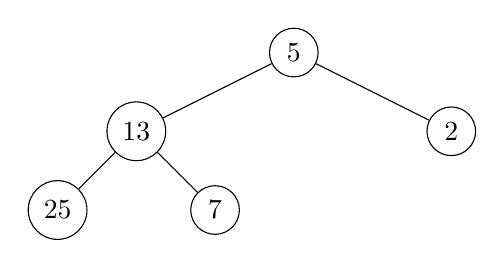
\begin{tikzpicture}[x=10mm, y=10mm]
	\node [circle, draw, fill=white] (1) at (0,0) {5};
	\node [circle, draw, fill=white] (2) at (-2,-1) {13};
	\node [circle, draw, fill=white] (3) at (2,-1) {2};
	\node [circle, draw, fill=white] (4) at (-3,-2) {25};
	\node [circle, draw, fill=white] (5) at (-1,-2) {7};
	\foreach \from/\to in {1/2, 1/3, 2/4, 2/5}
		\draw (\from) -- (\to);
\end{tikzpicture}

\

Then \verb|Min-Heapify| it.  

\

Find the min of these three, and swap it with the parent.  

\

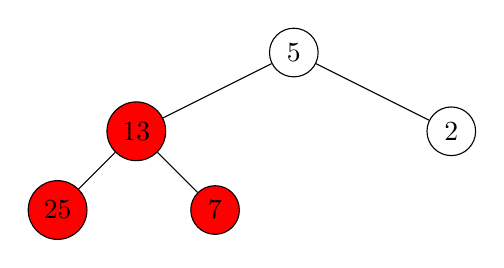
\begin{tikzpicture}[x=10mm, y=10mm]
	\node [circle, draw, fill=white] (1) at (0,0) {5};
	\node [circle, draw, fill=red] (2) at (-2,-1) {13};
	\node [circle, draw, fill=white] (3) at (2,-1) {2};
	\node [circle, draw, fill=red] (4) at (-3,-2) {25};
	\node [circle, draw, fill=red] (5) at (-1,-2) {7};
	\foreach \from/\to in {1/2, 1/3, 2/4, 2/5}
		\draw (\from) -- (\to);
\end{tikzpicture}

\
	
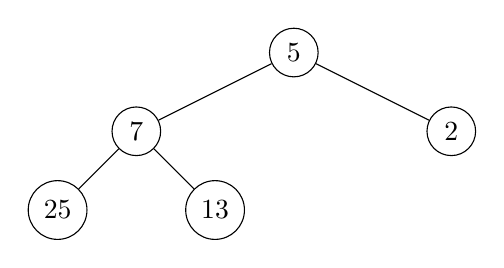
\begin{tikzpicture}[x=10mm, y=10mm]
	\node [circle, draw, fill=white] (1) at (0,0) {5};
	\node [circle, draw, fill=white] (2) at (-2,-1) {7};
	\node [circle, draw, fill=white] (3) at (2,-1) {2};
	\node [circle, draw, fill=white] (4) at (-3,-2) {25};
	\node [circle, draw, fill=white] (5) at (-1,-2) {13};
	\foreach \from/\to in {1/2, 1/3, 2/4, 2/5}
		\draw (\from) -- (\to);
\end{tikzpicture}

\

Find the min of these three, and swap it with the parent.  

\
	
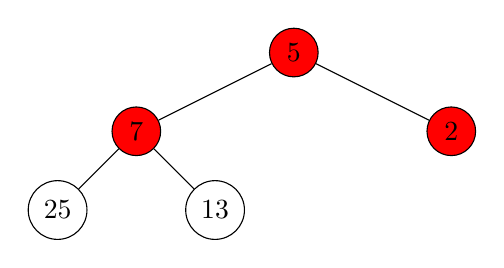
\begin{tikzpicture}[x=10mm, y=10mm]
	\node [circle, draw, fill=red] (1) at (0,0) {5};
	\node [circle, draw, fill=red] (2) at (-2,-1) {7};
	\node [circle, draw, fill=red] (3) at (2,-1) {2};
	\node [circle, draw, fill=white] (4) at (-3,-2) {25};
	\node [circle, draw, fill=white] (5) at (-1,-2) {13};
	\foreach \from/\to in {1/2, 1/3, 2/4, 2/5}
		\draw (\from) -- (\to);
\end{tikzpicture}

\

Now we have a min heap.  

\
	
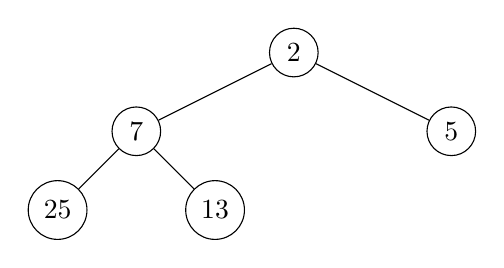
\begin{tikzpicture}[x=10mm, y=10mm]
	\node [circle, draw, fill=white] (1) at (0,0) {2};
	\node [circle, draw, fill=white] (2) at (-2,-1) {7};
	\node [circle, draw, fill=white] (3) at (2,-1) {5};
	\node [circle, draw, fill=white] (4) at (-3,-2) {25};
	\node [circle, draw, fill=white] (5) at (-1,-2) {13};
	\foreach \from/\to in {1/2, 1/3, 2/4, 2/5}
		\draw (\from) -- (\to);
\end{tikzpicture}

\

At each step, swap the root with the last leaf, decrement the number of elements in the heap (but not the array), and restore the min-heap using \verb|Min-Heapify|.  Repeat until the heap is empty.  

\

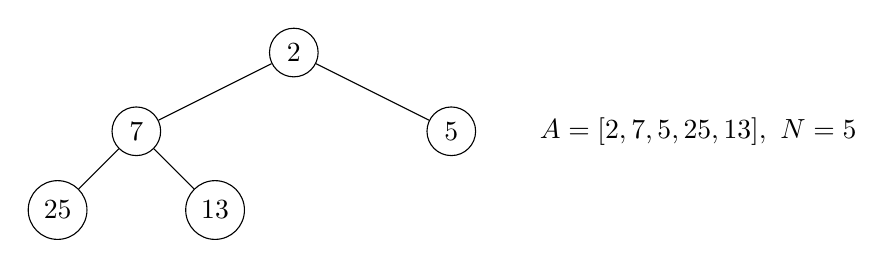
\begin{tikzpicture}[x=10mm, y=10mm]
	\node [circle, draw, fill=white] (1) at (0,0) {2};
	\node [circle, draw, fill=white] (2) at (-2,-1) {7};
	\node [circle, draw, fill=white] (3) at (2,-1) {5};
	\node [circle, draw, fill=white] (4) at (-3,-2) {25};
	\node [circle, draw, fill=white] (5) at (-1,-2) {13};
	\foreach \from/\to in {1/2, 1/3, 2/4, 2/5}
		\draw (\from) -- (\to);
	\node [right] () at (3,-1) {$A = [2,7,5,25,13], \ N=5$};
\end{tikzpicture}

\

Swap

\

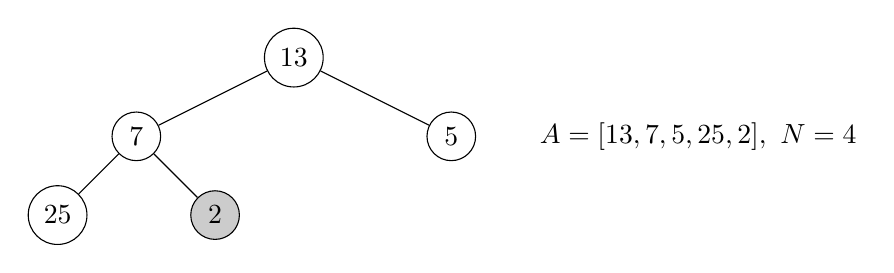
\begin{tikzpicture}[x=10mm, y=10mm]
	\node [circle, draw, fill=white] (1) at (0,0) {13};
	\node [circle, draw, fill=white] (2) at (-2,-1) {7};
	\node [circle, draw, fill=white] (3) at (2,-1) {5};
	\node [circle, draw, fill=white] (4) at (-3,-2) {25};
	\node [circle, draw, fill=white!80!black] (5) at (-1,-2) {2};
	\foreach \from/\to in {1/2, 1/3, 2/4, 2/5}
		\draw (\from) -- (\to);
	\node [right] () at (3,-1) {$A = [13,7,5,25,2], \ N=4$};
\end{tikzpicture}

\

Heapify

\

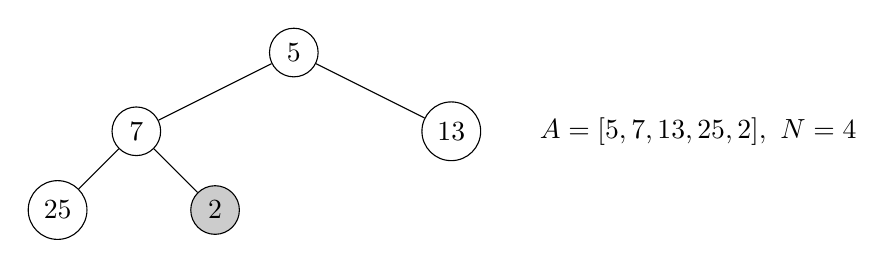
\begin{tikzpicture}[x=10mm, y=10mm]
	\node [circle, draw, fill=white] (1) at (0,0) {5};
	\node [circle, draw, fill=white] (2) at (-2,-1) {7};
	\node [circle, draw, fill=white] (3) at (2,-1) {13};
	\node [circle, draw, fill=white] (4) at (-3,-2) {25};
	\node [circle, draw, fill=white!80!black] (5) at (-1,-2) {2};
	\foreach \from/\to in {1/2, 1/3, 2/4, 2/5}
		\draw (\from) -- (\to);
	\node [right] () at (3,-1) {$A = [5,7,13,25,2], \ N=4$};
\end{tikzpicture}

\

Swap

\

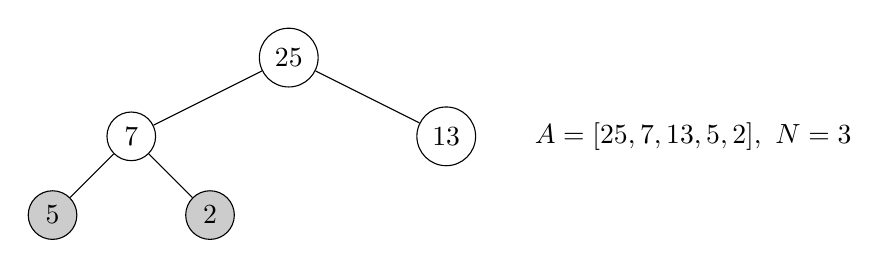
\begin{tikzpicture}[x=10mm, y=10mm]
	\node [circle, draw, fill=white] (1) at (0,0) {25};
	\node [circle, draw, fill=white] (2) at (-2,-1) {7};
	\node [circle, draw, fill=white] (3) at (2,-1) {13};
	\node [circle, draw, fill=white!80!black] (4) at (-3,-2) {5};
	\node [circle, draw, fill=white!80!black] (5) at (-1,-2) {2};
	\foreach \from/\to in {1/2, 1/3, 2/4, 2/5}
		\draw (\from) -- (\to);
	\node [right] () at (3,-1) {$A = [25,7,13,5,2], \ N=3$};
\end{tikzpicture}

\

Heapify

\

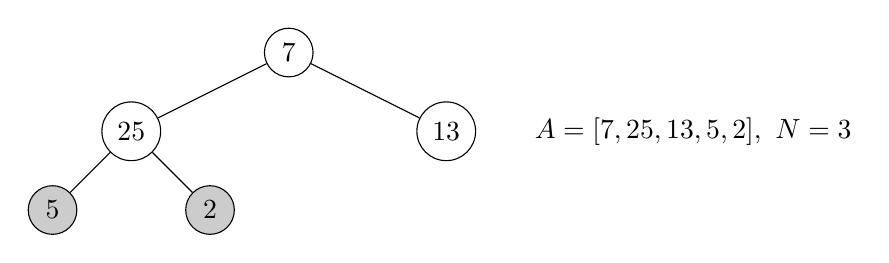
\begin{tikzpicture}[x=10mm, y=10mm]
	\node [circle, draw, fill=white] (1) at (0,0) {7};
	\node [circle, draw, fill=white] (2) at (-2,-1) {25};
	\node [circle, draw, fill=white] (3) at (2,-1) {13};
	\node [circle, draw, fill=white!80!black] (4) at (-3,-2) {5};
	\node [circle, draw, fill=white!80!black] (5) at (-1,-2) {2};
	\foreach \from/\to in {1/2, 1/3, 2/4, 2/5}
		\draw (\from) -- (\to);
	\node [right] () at (3,-1) {$A = [7,25,13,5,2], \ N=3$};
\end{tikzpicture}

\

Swap

\

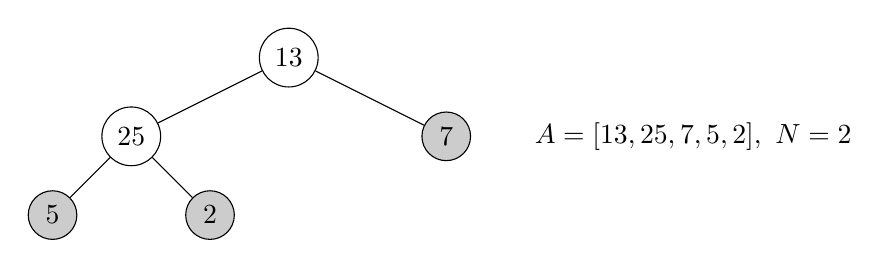
\begin{tikzpicture}[x=10mm, y=10mm]
	\node [circle, draw, fill=white] (1) at (0,0) {13};
	\node [circle, draw, fill=white] (2) at (-2,-1) {25};
	\node [circle, draw, fill=white!80!black] (3) at (2,-1) {7};
	\node [circle, draw, fill=white!80!black] (4) at (-3,-2) {5};
	\node [circle, draw, fill=white!80!black] (5) at (-1,-2) {2};
	\foreach \from/\to in {1/2, 1/3, 2/4, 2/5}
		\draw (\from) -- (\to);
	\node [right] () at (3,-1) {$A = [13,25,7,5,2], \ N=2$};
\end{tikzpicture}

\

Heapify (no change)

\

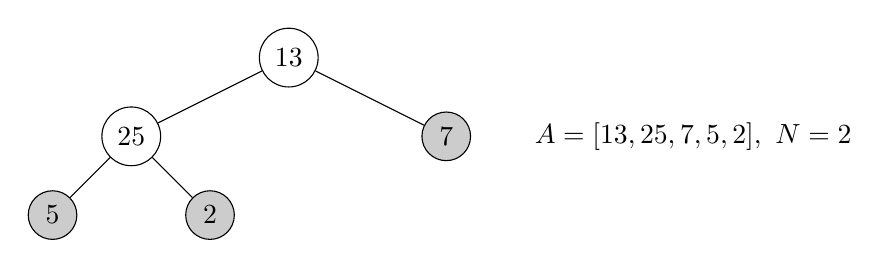
\begin{tikzpicture}[x=10mm, y=10mm]
	\node [circle, draw, fill=white] (1) at (0,0) {13};
	\node [circle, draw, fill=white] (2) at (-2,-1) {25};
	\node [circle, draw, fill=white!80!black] (3) at (2,-1) {7};
	\node [circle, draw, fill=white!80!black] (4) at (-3,-2) {5};
	\node [circle, draw, fill=white!80!black] (5) at (-1,-2) {2};
	\foreach \from/\to in {1/2, 1/3, 2/4, 2/5}
		\draw (\from) -- (\to);
	\node [right] () at (3,-1) {$A = [13,25,7,5,2], \ N=2$};
\end{tikzpicture}

\

Swap

\

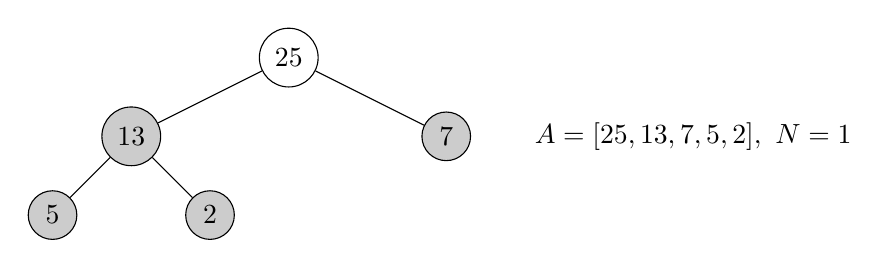
\begin{tikzpicture}[x=10mm, y=10mm]
	\node [circle, draw, fill=white] (1) at (0,0) {25};
	\node [circle, draw, fill=white!80!black] (2) at (-2,-1) {13};
	\node [circle, draw, fill=white!80!black] (3) at (2,-1) {7};
	\node [circle, draw, fill=white!80!black] (4) at (-3,-2) {5};
	\node [circle, draw, fill=white!80!black] (5) at (-1,-2) {2};
	\foreach \from/\to in {1/2, 1/3, 2/4, 2/5}
		\draw (\from) -- (\to);
	\node [right] () at (3,-1) {$A = [25,13,7,5,2], \ N=1$};
\end{tikzpicture}






